\chapter{Related Work}


boilerplate text, boilerplate text, boilerplate text, boilerplate text, boilerplate text, boilerplate text, boilerplate text, boilerplate text, boilerplate text, boilerplate text.


\section{Blockchain Basics}

The concept of a blockchain was introduced in the form of published hashes of data in newspaper format  \cite{whitakerArtBlockchainPrimer2019}

\subsection{Consensus Algorithms}

Proof-of-Work

Proof-of-Stake


\subsection{Oracles}



\subsection{Non-Fungible Tokens}

Created by crypto-kitties in 2018, specifically for art, but protocol can be used for other applications.


\section{Crypto-Art}


Early bitcoin inscribed ASCII artworks.

McCoy early work on Namecoin (2014)

Early work by Rhea Myers, predates NFTs.

Rhea Myers "Token Equals Text" (2019)


Tezos as the art chain (mention participation in basel

\section{Digital Art Preservation}

\subsection{NDSA Levels of Digital Preservation}


\begin{table}[h!]
\centering
\captionsetup{type=table} % This makes the caption be treated as a table caption
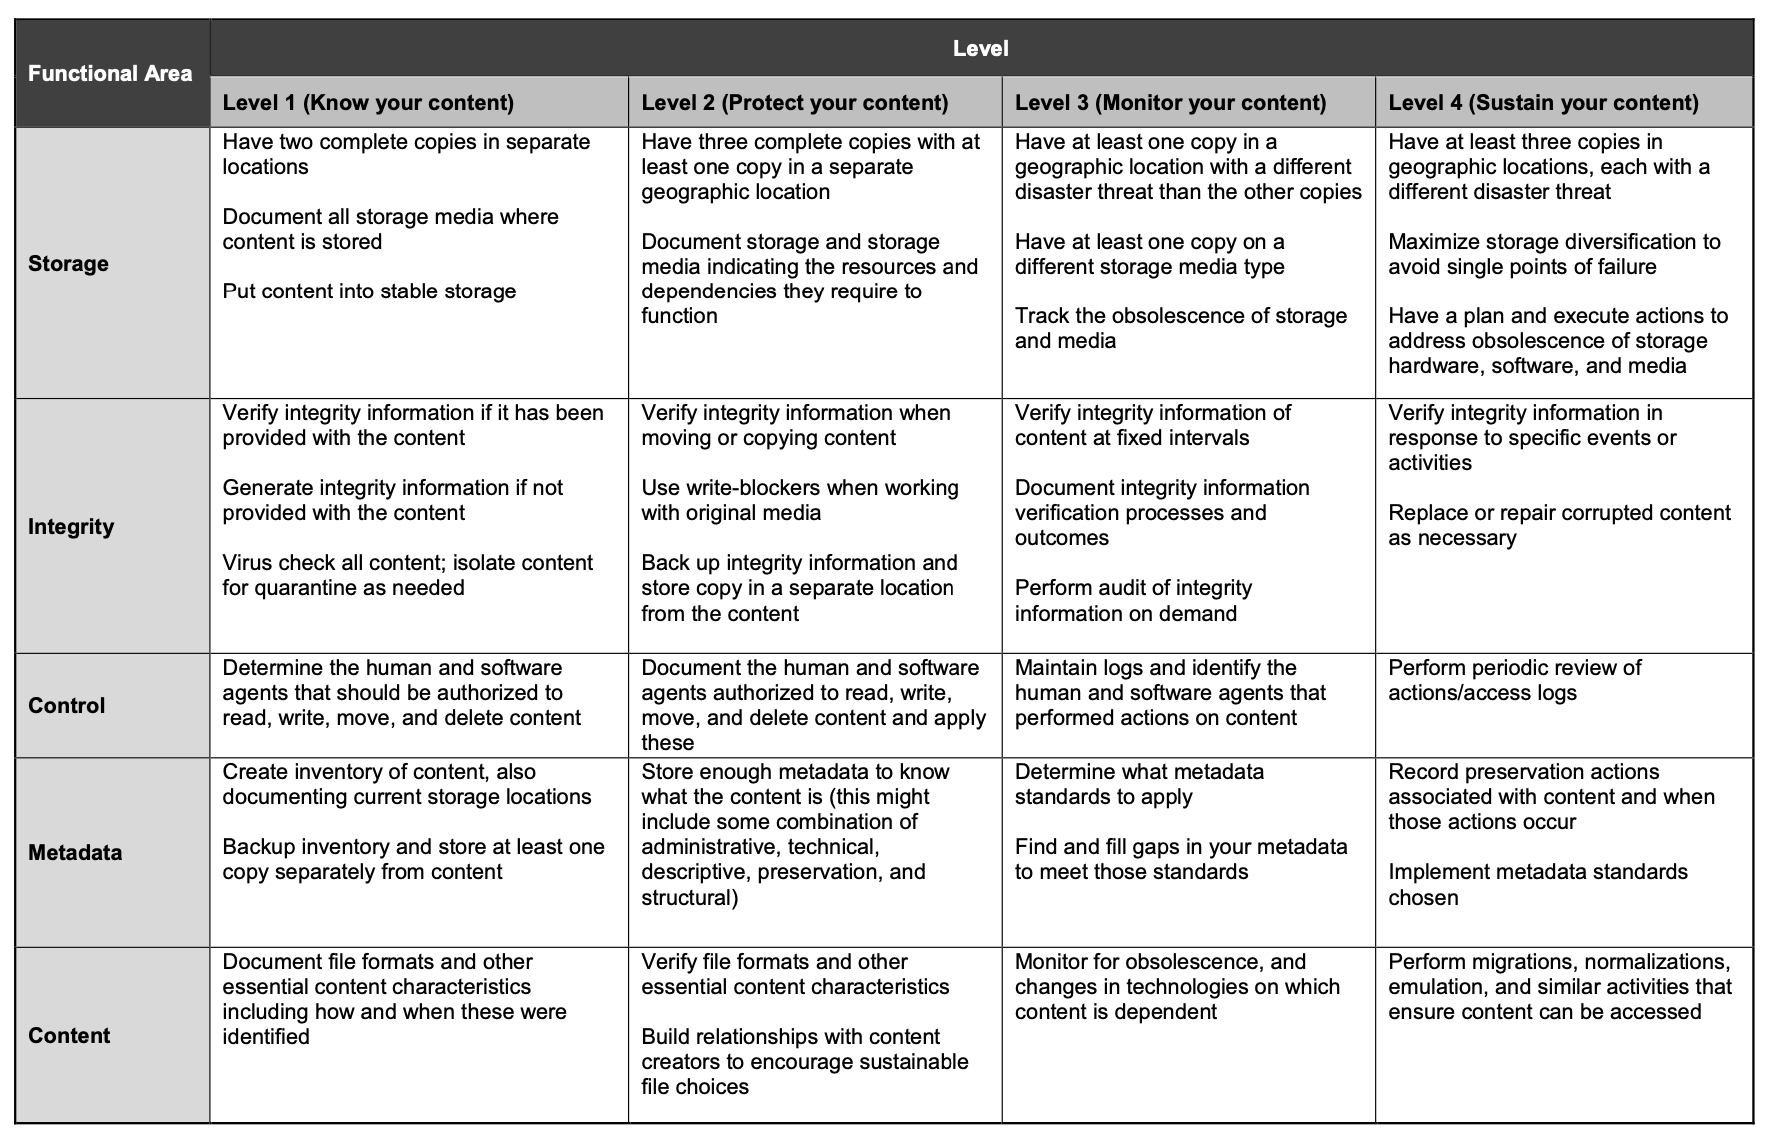
\includegraphics[width=\textwidth]{table-ndsa-matrix.png} % Adjust the width as needed
\caption[NDSA Levels of Digital Preservation Matrix V2.0]{NDSA Levels of Digital Preservation Matrix V2.0. Source: https://osf.io/qd54c}
\label{tab:ndsa-levels-of-digital-preservation}
\end{table}


\section{Web Archiving: State of the Art}

webrecorder
\subsection{Web Archiving Standards}

WARC


\section{Data Storage}

\subsection{On-Chain Storage}


mention fxhash articles (https://docs.fxhash.xyz/articles) and their tezos pointer scheme (https://github.com/fxhash/specifications/blob/main/general/tezos-storage-pointers.md) which may be useful for the idea of cross contract references, which is my plan for documentation (each person, one contract, cross-referecning OBJKTs)

\subsection{Interplanetary File System (IPFS)}

\subsection{Arweave}




\section{Provenance}

\subsection{Atomic Form}

Atomic Form combines the best of IPFS and Arweave into a single solution \cite{maneliusExtendingNFTMetadata2024}




\section{Interactivity}

\subsection{Self-Awareness}

\begin{figure}[h]
    \centering
    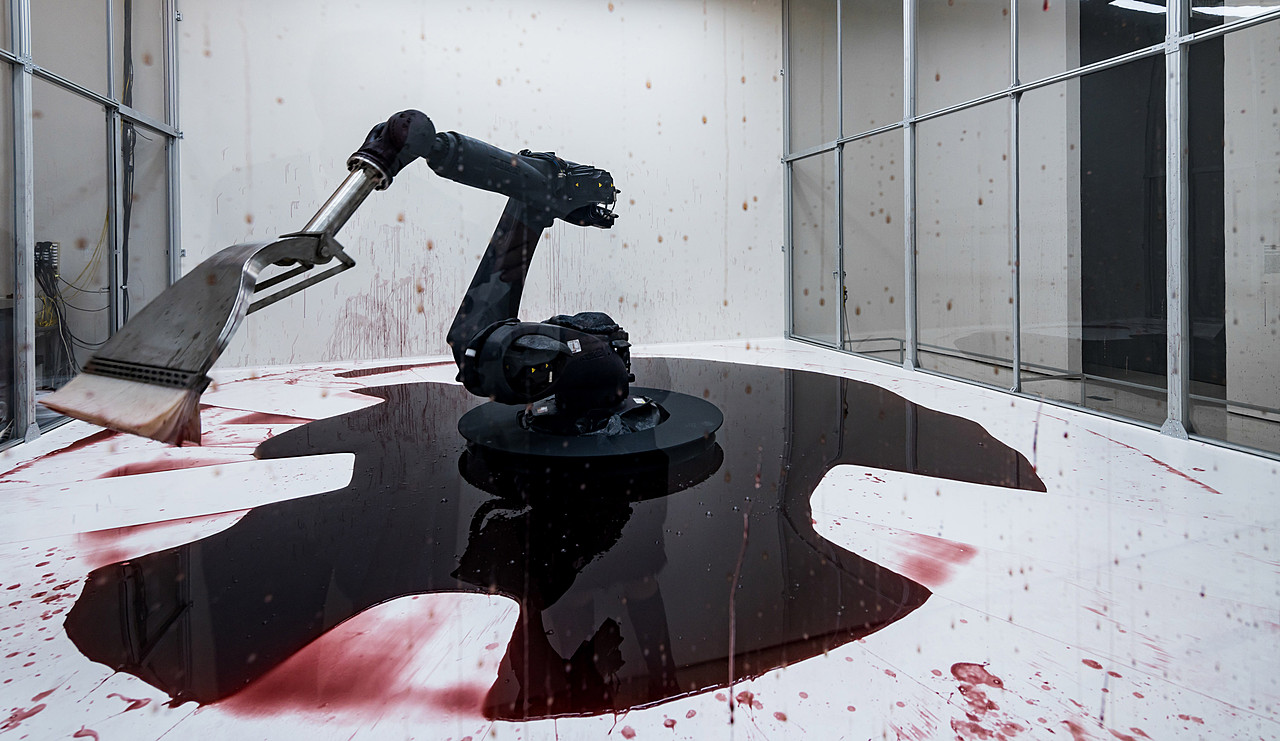
\includegraphics[width=\linewidth]{artwork-robot-cant-help.jpg}
    \caption[Can’t Help Myself by Sun Yuan \& Peng Yu]{Can’t Help Myself by Sun Yuan \& Peng Yu, 2016. Source: https://www.guggenheim.org/artwork/34812}
    \label{fig:robot-canthelp}
\end{figure}


This is a test reference to the work \cref{fig:robot-canthelp}

\subsection{Viewer Interactivity}

\subsection{Network Interactivity}

\subsection{Time Interactivity}


\subsection{LocalStorage Interactivity}

Entanglement by Bjork (have permission for screenshots)

\section{Determinism}

This section deals with whether artworks are deterministic in the way they are rendered or whether there is an element of randomness that even given all the same starting conditions, the artwork will look very different each time. This categorisation is important for conservation because a nondeterministic artwork will be dificult to monitor from a browser obsolescence point of view, especially when using image difference between consecutive snapshots of the artwork. In the case of a non-deterministic artwork, the snapshots will be so different that they become ineffective in detecting changes due to browser version upgrades or other changes in web specifications overtime. In this context, the challenge is to differentiate between a deterministic animated artwork, and a nondeterministic artwork. This challenge exists, because even if an artwork is deterministic, unless there is a way to snapshot the exact same frame across all the snapshots then any image difference comparisons will result in exaggerated differences. In this case we may need to employ more advanced animation frame comparison algorithms, such that the sequence of the animation can be compared across snapshots, and these may involve the recording of the animation, rather than just taking a single snapshot in time. Of course, such a strategy has trade-offs, and in this particular case the trade-off would be a much larger snapshot file size, which will then impact on the overall economic sustainability of the archive.


\section{Code Security}

In this section I review methods of detecting potential malicious code

Strategies can involve code similarity checks \cite{ragkhitwetsagulComparisonCodeSimilarity2018} and particularly in JavaScript \cite{alfagehCloneDetectionTechniques2020} where an artwork's code can be compared against well known wallet code.

This can also aid in identifying potential outdated libraries which could contain vulnerabilities or even current libraries which were attacked by hackers, looking to add backdoors or other crypto exploiting code.



\section{Blockchain as the Medium}

Mad Dog Jones Replicator (2021) - uses an off-chain server (under control of the artist) as an oracle which sends "paper-jam" events to the artwork's smart contract.

\section{Decentralisation}
\label{sec:lit_review:decentralisation}

\section{Main Issues}

\subsection{Scalability}

One key aspect to remember is that adding more nodes to a network does not improve network scalability if each node must replicate the exact same computation as every other node, which is the case with most consensus and block validating nodes on a blockchain. Of course such wide replication of computation is still desired, for decentralisation purposes, as discussed in \ref{sec:lit_review:decentralisation}


\subsubsection{Moore's Law and Data Storage}

\section{Economic Sustainability}

mention VDP, its role in wg3.2 (beneficiaries), and how the idea spread to other marketplaces (https://docs.fxhash.xyz/pricing-and-supply)



